\documentclass[10pt,a4paper]{article}
\usepackage[margin=21mm,headheight=15pt]{geometry}
\usepackage[T1]{fontenc}
\usepackage{lmodern,amsmath,amssymb,tikz,graphicx,hyperref,fancyhdr,enumitem}
\usetikzlibrary{arrows.meta,positioning,calc,decorations.pathmorphing}
\definecolor{ink}{RGB}{20,53,78}
\hypersetup{colorlinks=true,urlcolor=ink,linkcolor=ink}
\setlength{\parindent}{0pt}\setlength{\parskip}{5pt}
\emergencystretch=3em
\pagestyle{fancy}\fancyhf{}\fancyfoot[C]{\thepage}
\renewcommand{\headrulewidth}{.3pt}
\newcommand{\task}[2]{\par\medskip{\color{ink}\Large\bfseries #1. #2}\par\smallskip}
\newcommand{\answer}{\par\smallskip\textbf{Worked reasoning.} }
\setlist[enumerate]{label=\textbf{(\alph*)},leftmargin=7mm,itemsep=7pt}
\begin{document}
\fancyhead[L]{\small Control of Dynamical Systems}
\fancyhead[R]{\small Laboratory 10}
{\color{ink}\LARGE\bfseries Laboratory 10}\par
{\large Two thermal zones with one temperature measurement}\par
\textbf{Exercise sheet -- five integrated problems}\par
{\small\textbf{Evidence boundary.} Original hypothetical scenarios. Derive, calculate and justify decisions; every numerical record is synthetic. Figures are conceptual and not to scale.}
\smallskip\textbf{Shared nominal data.} Two-zone model: $A=[-0.15,0.05;\,0.05,-0.10]$, $B=[0.1,0]^{\mathsf T}$ and $C=[0,1]$. Feedback pole targets are $-0.20,-0.35$ s$^{-1}$ and observer targets are $-0.8,-1.0$ s$^{-1}$.
\task{1}{Two thermal zones, one heater and one thermometer}
The illustration shows two lumped thermal masses coupled by a conductive bridge. Only zone 1 is heated and only zone 2 is measured.
\begin{center}\resizebox{\ifdim\width>.98\linewidth.98\linewidth\else\width\fi}{!}{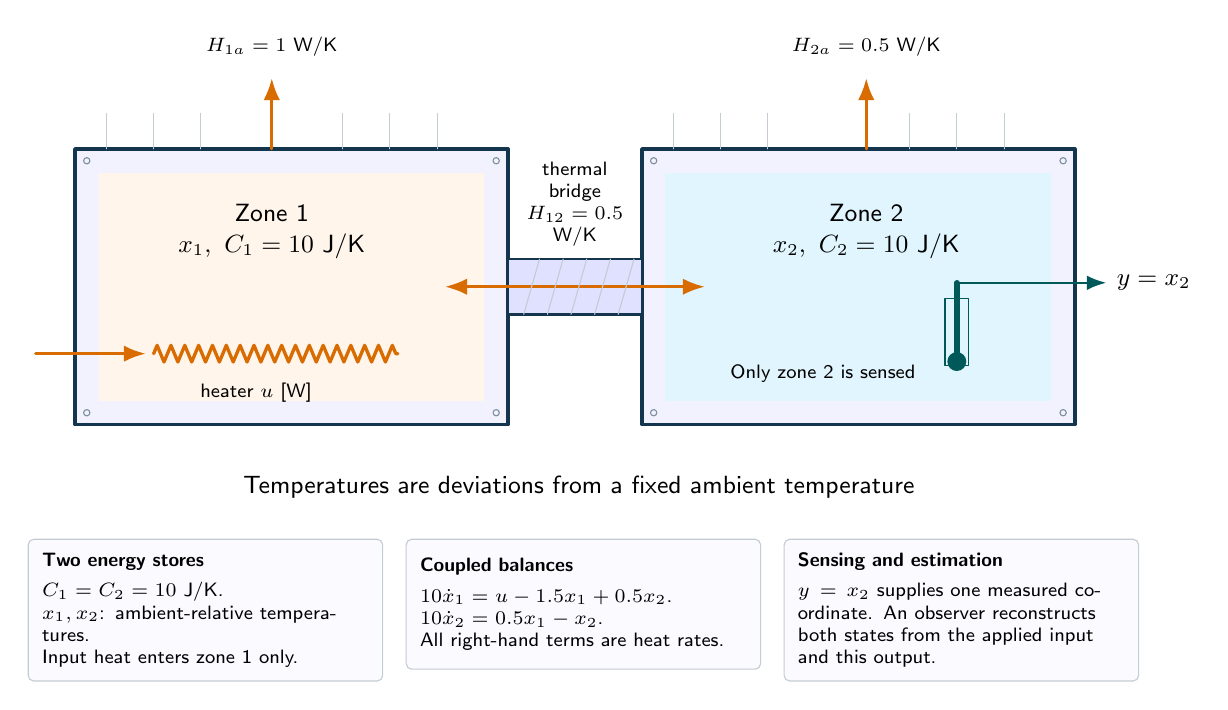
\begin{tikzpicture}[
font=\sffamily\small,>=Latex,line cap=round,line join=round,
wall/.style={draw=ink,line width=1.2pt,fill=blue!5},
water/.style={fill=cyan!25,draw=none},
metal/.style={draw=ink,fill=blue!12,line width=.9pt},
flow/.style={->,draw=blue!65!black,line width=1.2pt},
heat/.style={->,draw=orange!85!black,line width=1.1pt},
measure/.style={->,draw=teal!70!black,line width=.9pt},
dim/.style={<->,draw=ink!65,line width=.6pt},
spring/.style={draw=ink,decorate,decoration={coil,aspect=.5,segment length=4pt,amplitude=3pt}},
wire/.style={draw=ink,line width=1pt},
lab/.style={align=center,font=\sffamily\small},
smalllab/.style={align=center,font=\sffamily\scriptsize}]

\draw[wall](.6,.7)rectangle(6.1,4.2);
\draw[wall](7.8,.7)rectangle(13.3,4.2);
\fill[orange!8](.9,1)rectangle(5.8,3.9);
\fill[cyan!12](8.1,1)rectangle(13,3.9);
\draw[metal](6.1,2.1)rectangle(7.8,2.8);
\draw[heat,<->](5.3,2.45)--(8.6,2.45);
\node[smalllab]at(6.95,3.5){thermal\\bridge\\$H_{12}=0.5$\\W/K};
\draw[orange!85!black,line width=1.2pt,decorate,decoration={zigzag,segment length=5pt,amplitude=3pt}](1.6,1.6)--(4.7,1.6);
\draw[heat](.1,1.6)--(1.5,1.6);
\node[smalllab]at(2.9,1.1){heater $u$ [W]};
\node[lab]at(3.1,3.15){Zone 1\\$x_1,\ C_1=10$ J/K};
\node[lab]at(10.65,3.15){Zone 2\\$x_2,\ C_2=10$ J/K};
\draw[teal!70!black,line width=2pt](11.8,1.5)--(11.8,2.5);
\fill[teal!70!black](11.8,1.5)circle(.12);
\draw[measure](11.8,2.5)--(13.7,2.5)node[right]{$y=x_2$};
\draw[heat](3.1,4.2)--(3.1,5.1);
\draw[heat](10.65,4.2)--(10.65,5.1);
\node[smalllab]at(3.1,5.5){$H_{1a}=1$ W/K};
\node[smalllab]at(10.65,5.5){$H_{2a}=0.5$ W/K};
\node[lab]at(7,-.1){Temperatures are deviations from a fixed ambient temperature};
% REFINED EQUIPMENT DETAILS

% Distinct thermal masses and finite conductive contact.
\foreach \x in {1,1.6,2.2,4,4.6,5.2}{\draw[ink!25](\x,4.2)--(\x,4.65);}
\foreach \x in {8.2,8.8,9.4,11.2,11.8,12.4}{\draw[ink!25](\x,4.2)--(\x,4.65);}
\foreach \x in {6.3,6.6,6.9,7.2,7.5}{\draw[ink!25](\x,2.1)--(\x+.2,2.8);}
\foreach \x/\y in {.75/.85,.75/4.05,5.95/.85,5.95/4.05,7.95/.85,7.95/4.05,13.15/.85,13.15/4.05}{\draw[ink!55](\x,\y)circle(.04);}
\draw[teal!70!black](11.65,1.45)rectangle(11.95,2.3);
\node[smalllab]at(10.1,1.35){Only zone 2 is sensed};

\node[draw=ink!25,fill=blue!2,rounded corners=2pt,anchor=north west,text width=4.15cm,minimum height=1.65cm,inner sep=5pt,align=left,font=\sffamily\scriptsize]at(0.0,-0.75){\textbf{Two energy stores}\\[3pt]$C_1=C_2=10$ J/K.\\$x_1,x_2$: ambient-relative temperatures.\\Input heat enters zone 1 only.};
\node[draw=ink!25,fill=blue!2,rounded corners=2pt,anchor=north west,text width=4.15cm,minimum height=1.65cm,inner sep=5pt,align=left,font=\sffamily\scriptsize]at(4.8,-0.75){\textbf{Coupled balances}\\[3pt]$10\dot x_1=u-1.5x_1+0.5x_2$.\\$10\dot x_2=0.5x_1-x_2$.\\All right-hand terms are heat rates.};
\node[draw=ink!25,fill=blue!2,rounded corners=2pt,anchor=north west,text width=4.15cm,minimum height=1.65cm,inner sep=5pt,align=left,font=\sffamily\scriptsize]at(9.6,-0.75){\textbf{Sensing and estimation}\\[3pt]$y=x_2$ supplies one measured coordinate. An observer reconstructs both states from the applied input and this output.};
\end{tikzpicture}
}\par{\small Two thermal inventories are connected by a conductive bridge. Heating acts in the first zone and sensing in the second. These stated capacities and conductances reproduce the two-state model exactly under the lumped assumptions.}\end{center}
\begin{enumerate}
\item Consider $A=[-0.15,0.05;0.05,-0.10]$, $B=[0.1,0]^T$, $C=[0,1]$. Write both scalar state equations and identify the actuated and measured zones. Find the open-loop poles.
\item Construct the controllability and observability matrices and evaluate their determinants. Explain the role of inter-zone coupling.
\item Realize the stated matrix using $C_1=C_2=10$ J/K, coupling conductance $H_{12}=0.5$ W/K and ambient conductances $H_{1a}=1$, $H_{2a}=0.5$ W/K. Derive the balances and explain what happens to controllability and observability when coupling is removed.
\end{enumerate}
\vfill{\small\textbf{Submission.} Show the model, intermediate reasoning, units and a conclusion addressing the stated requirements.}

\newpage
\task{2}{Pole placement and the distinction between transient and steady feasibility}
First design ideal full-state feedback and its reference prefilter. Then check whether the resulting input request can be delivered by a constrained heater.
\begin{enumerate}
\item Choose $u=-Kx+Nr$ so $A-BK$ has poles $-0.2$ and $-0.35$. Derive K by matching trace and determinant, without a pole-placement library.
\item With $K=[3,5.5]$, find N for unit DC reference tracking at $y=x_2$. Determine both equilibrium states and input for a unit reference.
\item Use $r=0.5$, zero initial states and heater limits $0\le u\le2$ W. Compare the immediate ideal control request with the equilibrium request. Does a feasible equilibrium imply an entirely unsaturated transient?
\end{enumerate}
\vfill{\small\textbf{Submission.} Show the model, intermediate reasoning, units and a conclusion addressing the stated requirements.}

\newpage
\task{3}{An observer must receive the input actually applied}
Construct the observer and analyze estimated-state feedback. Distinguish the linear separation argument from an implementation with actuator clipping.
\begin{center}\resizebox{\ifdim\width>.98\linewidth.98\linewidth\else\width\fi}{!}{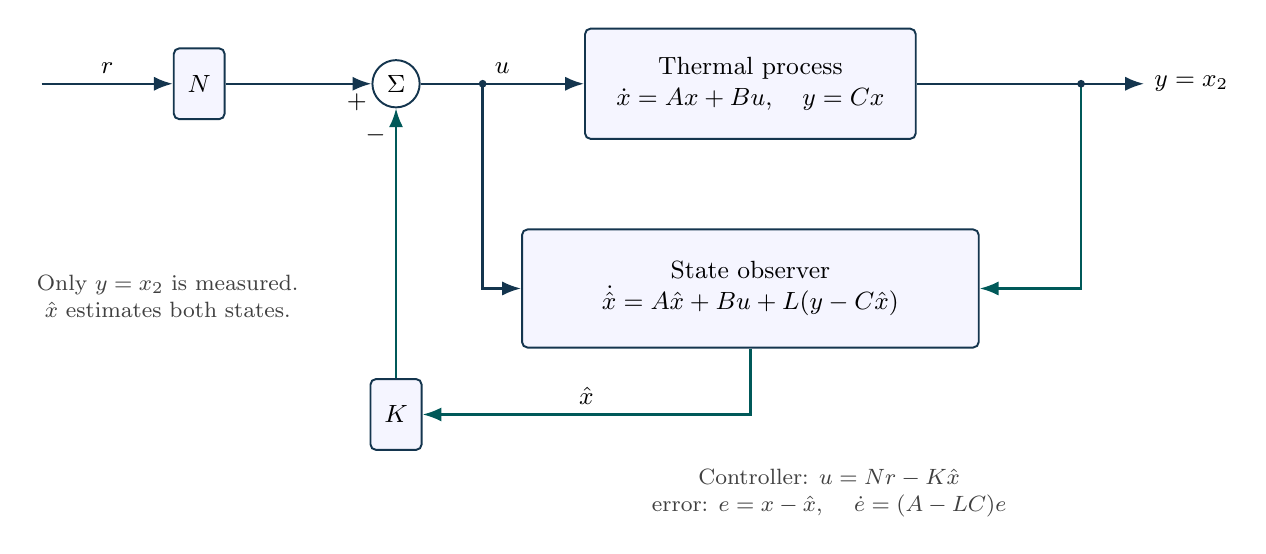
\begin{tikzpicture}[x=1cm,y=1cm,>=Latex,font=\small,
block/.style={draw=ink,fill=blue!4,rounded corners=2pt,minimum height=9mm,align=center,line width=.7pt,inner sep=5pt},
sum/.style={circle,draw=ink,fill=white,minimum size=6mm,inner sep=0pt,line width=.7pt},
sig/.style={->,draw=ink,line width=.85pt},
fb/.style={->,draw=teal!70!black,line width=.85pt},
dist/.style={->,draw=orange!75!black,line width=.85pt},
tap/.style={circle,fill=ink,inner sep=1.4pt},
note/.style={font=\footnotesize,align=center,text=black!75}]

\node[block](n)at(2,1.1){$N$};
\node[sum](u)at(4.5,1.1){$\Sigma$};
\node[block,minimum width=42mm,minimum height=14mm](p)at(9,1.1){Thermal process\\$\dot x=Ax+Bu,\quad y=Cx$};
\draw[sig](0,1.1)--node[above]{$r$}(n);
\draw[sig](n)--node[pos=.9,below]{$+$}(u);
\draw[sig](u)--node[above]{$u$}(p);
\draw[sig](p)--(14,1.1)node[right]{$y=x_2$};
\node[block,minimum width=58mm,minimum height=15mm](o)at(9,-1.5){State observer\\$\dot{\hat x}=A\hat x+Bu+L(y-C\hat x)$};
\draw[sig](5.6,1.1)--(5.6,-1.5)--(o.west);
\fill[ink](5.6,1.1)circle(1.4pt);
\draw[fb](13.2,1.1)--(13.2,-1.5)--(o.east);
\fill[ink](13.2,1.1)circle(1.4pt);
\node[block](k)at(4.5,-3.1){$K$};
\draw[fb](o.south)--(9,-3.1)--node[above]{$\hat x$}(k);
\draw[fb](k.north)--node[pos=.9,left]{$-$}(u.south);
\node[note]at(1.6,-1.6){Only $y=x_2$ is measured.\\$\hat x$ estimates both states.};
\node[note]at(10,-4.1){Controller: $u=Nr-K\hat x$\\error: $e=x-\hat x$, $\quad\dot e=(A-LC)e$};

\end{tikzpicture}
}\par{\small The observer receives both the applied control and measured output. Its estimated vector supplies state feedback; the prefilter sets nominal reference gain.}\end{center}
\begin{enumerate}
\item Use $\dot{\hat x}=A\hat x+Bu+L(y-C\hat x)$ and place observer error poles at $-0.8$ and $-1$. Derive both entries of L.
\item With estimated-state control $u=-K\hat x+Nr$, derive the augmented dynamics in coordinates $[x,e]$ where $e=x-\hat x$. List all four eigenvalues and state the assumptions.
\item If the heater saturates, derive the estimation-error dynamics when the observer receives actual applied $u$. Contrast this with feeding it the unlimited request $u_*$. State which linear conclusion no longer follows automatically.
\end{enumerate}
\vfill{\small\textbf{Submission.} Show the model, intermediate reasoning, units and a conclusion addressing the stated requirements.}

\newpage
\task{4}{Unknown heat leakage, actuator capacity and integral augmentation}
A constant unmodeled heat input enters zone 2. The nominal reference prefilter cannot cancel an unknown disturbance, and additional control action still faces a finite heater limit.
\begin{enumerate}
\item For full-state feedback with the nominal prefilter, add disturbance $d$ to $\dot x_2$. Derive the final output error for a constant d and evaluate it at $d=0.01$.
\item Assume heater command must stay in $[0,2]$. Under the nominal model, determine the largest positive constant zone-2 reference that full-state control can maintain at equilibrium. Explain the implication for a requested reference of one.
\item Propose an integral state for rejecting an unknown constant output error and write the augmented plant matrices before gain design. Check whether the nominal augmented model is controllable, and explain what augmentation cannot fix.
\end{enumerate}
\vfill{\small\textbf{Submission.} Show the model, intermediate reasoning, units and a conclusion addressing the stated requirements.}

\newpage
\task{5}{Fast estimation, biased sensors and the limits of a noise-path calculation}
Observer poles are chosen faster than controller poles. Examine both modal time scales and the effect of measurement noise without claiming that faster poles improve every error norm.
\begin{enumerate}
\item Let measured output be $y_m=Cx+n$. Derive the estimation-error dynamics with noise. Then, with true state and input held at zero, derive the transfer from n to the estimate of zone 2 for the selected observer.
\item Compare the slowest controller and observer modal time constants. Explain why a faster observer pole does not by itself guarantee the same proportional decrease in every estimation-error norm at every time.
\item Hold the true state and input at zero and add constant sensor bias $n=0.1$ K. Find both steady state estimates for the chosen observer. Explain why this open estimator test does not directly give the final output of the fully closed loop.
\end{enumerate}
\vfill{\small\textbf{Submission.} Show the model, intermediate reasoning, units and a conclusion addressing the stated requirements.}

\end{document}
